%% ============================================================================
%% ICAIF-style paper (ACM sigconf). Full version: complete story in the body,
%% every experiment retained (supporting detail in the appendices).
%%
%% FONTS / SIZES / LAYOUT are fixed by the ACM `acmart' class with `sigconf'
%% (two-column, 9pt Libertine body, ACM heading sizes). ACM forbids changing
%% them, so we do NOT set \fontsize / geometry / column widths by hand.
%% Do not add \usepackage{times}, \geometry, or manual font-size commands.
%%
%% COMPILE: Overleaf ("ACM Conference Proceedings (acmart)") or a TeX Live /
%% tectonic with the `acmart' package. `nonacm' suppresses the copyright strip
%% for a working draft; remove it and fill \acm* metadata for camera-ready.
%% For the ICAIF main track add `anonymous' to the class options.
%% ============================================================================
\documentclass[sigconf,nonacm]{acmart}

\settopmatter{printacmref=false}
\setcopyright{none}
\renewcommand\footnotetextcopyrightpermission[1]{}

\usepackage{booktabs}
\usepackage{graphicx}
\usepackage{xurl}                    % break long URLs at any character (never exceed the column)
\setlength{\emergencystretch}{3em}   % let TeX stretch spacing as a last resort rather than
                                     % overflow the right margin -- lines wrap instead of running over

\begin{document}

\title{Magnitude, Not Shape: Volatility Beats Downside- and Tail-Risk
Metrics at Forecasting Drawdown}

\author{Meghanadh Pulivarthi}
% \affiliation{%
%   \institution{Independent Researcher}
%   \country{}}
\email{meghanadh27@gmail.com}
\renewcommand{\shortauthors}{Pulivarthi}

\begin{abstract}
Every few years a new downside- or tail-risk metric is proposed to improve on
plain return volatility. The premise is always the same. The \emph{shape} of the
loss distribution, whether its asymmetry, tail heaviness, or co-crash structure, is
supposed to carry information that symmetric volatility misses. We test that premise
as adversarially as the data allow. On a survivorship-free, multi-regime,
multiple-testing-corrected evaluation of ten metrics across five test beds, no
metric reliably beats volatility at forecasting an asset's forward maximum drawdown,
whether the metric is published or machine-discovered. The failure has a clean
anatomy, which we call \emph{magnitude, not shape}. The partial rank correlation of
Value-at-Risk with forward drawdown, controlling for volatility, survives
Benjamini--Hochberg correction on all five beds, though it reaches only $0.19$ at
its largest. Every tail-\emph{shape} metric adds nothing or subtracts. The shape metrics are not broken. On genuinely
shape-sensitive targets they beat volatility. Drawdown is simply a magnitude
phenomenon that shape does not drive. Volatility is
hard to beat because it is persistent, but a predictive mediation test shows it is
not a sufficient statistic. The tiny magnitude edge is not economically free either.
A cost-aware backtest and a pre-registered composite add nothing over volatility
except in fat-tailed crypto. Finally, an autonomous large-language-model discovery
loop only inflates validation while its locked-test score plateaus at volatility, a
data-snooping caution now that agentic search makes signal-hunting nearly free.
Volatility is not glamorous, but on a level field it is very hard to beat.
\end{abstract}

\begin{CCSXML}
<ccs2012>
<concept><concept_id>10010147.10010257</concept_id>
<concept_desc>Computing methodologies~Machine learning</concept_desc>
<concept_significance>500</concept_significance></concept>
<concept><concept_id>10003752.10010070</concept_id>
<concept_desc>Applied computing~Economics</concept_desc>
<concept_significance>500</concept_significance></concept>
</ccs2012>
\end{CCSXML}
\ccsdesc[500]{Computing methodologies~Machine learning}
\ccsdesc[500]{Applied computing~Economics}

\keywords{downside risk, tail risk, drawdown, volatility, survivorship bias,
multiple testing, data snooping, LLM agents}

\maketitle

%% =========================================================================
\section{Introduction}
Prices fall faster than they rise, and it is the fall that ruins investors. From
that intuition a large literature has grown. It proposes metrics that look past
symmetric volatility to the \emph{shape} of the loss distribution. These include
lower partial moments and the Sortino ratio~\cite{bawa1975,fishburn1977,sortino1991},
the partial-moment ``predictive'' ratio~\cite{violenawrocki2016}, left-tail
Value-at-Risk and expected shortfall~\cite{rockafellar2000,atilgan2020}, realized
semibetas~\cite{bpq2022}, downside beta~\cite{ang2006,leviwelch2020}, lower-tail
dependence~\cite{chabiyo2018}, disappointment-aversion risk~\cite{faragotedongap2018},
and tail-exponent factors~\cite{kellyjiang2014}. Each rests on the same premise, that
asymmetry or tail structure carries information volatility misses.

We test that premise on the fairest field we can build. Three disciplines the
source literature usually omits turn out to matter enormously. A
\emph{survivorship-free} universe keeps the assets that actually died. A
\emph{locked} out-of-sample holdout stops search from leaking into the verdict. And
\emph{multiple-testing correction} keeps an evaluation of dozens of comparisons from
manufacturing winners. We evaluate ten metrics, volatility and nine downside- and
tail-risk challengers, as forecasters of $90$-day forward
maximum drawdown across five cross-sectional test beds spanning calm, bull, and
crash regimes in crypto and equity, with per-date rank correlations, paired
block-bootstrap confidence intervals, and Benjamini--Hochberg (BH) correction.

The headline is negative and, in hindsight, unsurprising. No metric reliably beats
plain volatility. Our contribution is the \emph{anatomy} of that result and the
honesty of the battery behind it. (1) A clean empirical law we call \emph{magnitude,
not shape}. The only signal surviving correction beyond volatility is the \emph{size}
of tail losses (VaR/ES/downside deviation), not their asymmetry (\S\ref{sec:magnitude}).
(2) Volatility is hard to beat because it is \emph{persistent}, though a predictive
test shows forward volatility is not a sufficient statistic (\S\ref{sec:why}). (3) The
residual edge is not economically free, except in fat-tailed crypto (\S\ref{sec:why}).
(4) An autonomous large-language-model (LLM) discovery loop cannot beat volatility
out-of-sample and only overfits validation, a data-snooping caution as agentic
search makes signal-hunting nearly free (\S\ref{sec:why}). Every experiment is
retained, and supporting detail is in the appendices.

\textbf{Related work.} Lower partial moments generalize semi-variance~\cite{bawa1975,fishburn1977}
and underpin the Sortino ratio~\cite{sortino1991} and the partial-moment
ratio~\cite{violenawrocki2016}; tail measures include VaR/ES~\cite{rockafellar2000,atilgan2020},
semibetas~\cite{bpq2022}, downside beta~\cite{ang2006,leviwelch2020}, lower-tail
dependence~\cite{chabiyo2018}, disappointment aversion~\cite{faragotedongap2018}, and
tail exponents~\cite{kellyjiang2014}. Most were built to \emph{price} the cross-section,
not forecast one asset's drawdown; a separate literature studies the drawdown statistic
directly~\cite{magdonismail2004,chekhlov2005}. Volatility itself is a persistent,
tradable risk signal~\cite{moreiramuir2017,frazzinipedersen2014}. That volatility is
persistent is the founding fact of ARCH/GARCH~\cite{engle1982,bollerslev1986,andersen2003,corsi2009}; that searching
many signals inflates in-sample rank correlations is classical data
snooping~\cite{white2000,harvey2016,bailey2014,bailey2017}. Our novelty is to show an
\emph{autonomous} agent reaches the snooping frontier at near-zero cost.

%% =========================================================================
\section{Experimental Setup}\label{sec:data}
\textbf{Five test beds.} \emph{Crypto (survivorship-free):} a CoinMarketCap daily
panel (2013--2018) that retains crashed and delisted coins, so a point-in-time
top-$100$-by-market-cap universe includes assets that later crater; we use three
regimes: 2016 (calm), 2017 (bull), 2018 (crash). \emph{Equity:} S\&P~500
constituents, 1994--1999 (calm) and 2005--2009 (GFC). The equity beds are
survivorship-biased by construction (freely available equity data retains
almost no true deaths, itself a telling finding), so the survivorship claim
rests on the crypto beds, while equity tests cross-asset generality. We checked this
directly. A public, delisting-reputed price dump (the Kaggle Huge Stock Market dataset)
contains none of our windows' famous S\&P~500 casualties, with Lehman, Bear Stearns,
Enron, and WorldCom all absent, and yields zero mid-window delistings, so no free-data
equity bed we could build is genuinely survivorship-free.

\textbf{What we forecast.} From a $180$-day trailing window we forecast each asset's
$90$-day forward maximum drawdown, coding a delisting as a $-100\%$ loss. We score a
metric by its per-date cross-sectional rank correlation with that drawdown, averaged
over the bed, cross-sectional rather than time-series because the operational
question is which assets to derisk on a given date. 
% The remaining machinery
% (block-bootstrap confidence intervals, multiple-testing correction, the partial rank
% correlation, the discovery split, and what was pre-registered) is introduced where
% it first bites, below.

%% =========================================================================
\section{The verdict: nothing beats volatility}\label{sec:verdict}
The verdict is blunt. No metric beats volatility in a way that
survives a change of asset class. Table~\ref{tab:h2h} ranks each metric against
volatility standalone, with significance from paired block-bootstrap $95\%$ intervals
and Benjamini--Hochberg (BH) correction at $q=0.05$ applied within each family
(head-to-head and partials, ${\sim}45$ cells each). The block bootstrap uses length-$3$
blocks over the per-date series. On the thin crypto beds ($7$--$9$ dates) this grid is
coarse, so we back every crypto star with its interval and minimum detectable effect
(App.~\ref{app:partials}) and read crypto-only significance as suggestive. The only
metrics that significantly beat volatility on
\emph{any} bed are two volatility variants, downside deviation and VaR, on the single
crypto-bull bed, and both reverse on equity, where volatility significantly beats them.
Every genuinely different, shape-based metric is significantly \emph{worse} than
volatility on every bed.

We fix the bar in advance to avoid a moving goalpost. An edge counts as
\emph{generalizable} only if a metric BH-significantly beats volatility on at least one
crypto \emph{and} one equity bed, i.e., survives a change of asset class. No metric
clears it. Small, regime-specific edges exist for volatility's own variants, but none
survives a change of asset class. We pre-registered the main tests, fixing them before
we saw any results so they cannot be cherry-picked, namely the verdict, the
magnitude-versus-shape increments, and the composite. The finer slices by market stress
and across beds were explored afterward and count only as suggestive.

\begin{table}[t]
\centering
\caption{Standalone out-of-sample drawdown-forecast Spearman correlation.
$\ast$ = significantly beats volatility, $\dagger$ = significantly worse (both
survive BH, $q=0.05$); unmarked = indistinguishable. The Hill tail
exponent~\cite{kellyjiang2014} is omitted here (not estimable per date on
equity); its increment appears in Table~\ref{tab:partials}. Bold marks the highest value in each column.}
\label{tab:h2h}
\small
\begin{tabular}{lccccc}
\toprule
Metric & cr-16 & cr-17 & cr-18 & eq 94 & eq 05 \\
\midrule
\textbf{volatility} (base) & \textbf{0.62} & 0.36 & 0.38 & \textbf{0.61} & \textbf{0.56} \\
downside deviation & \textbf{0.62} & 0.38$\ast$ & \textbf{0.41} & 0.58$\dagger$ & 0.54$\dagger$ \\
VaR & 0.61 & \textbf{0.40}$\ast$ & 0.36 & 0.58$\dagger$ & 0.54$\dagger$ \\
ES~\cite{rockafellar2000} & \textbf{0.62} & 0.35 & 0.33$\dagger$ & 0.58$\dagger$ & 0.52$\dagger$ \\
neg.\ semibeta~\cite{bpq2022} & 0.40$\dagger$ & 0.26$\dagger$ & 0.31$\dagger$ & 0.49$\dagger$ & 0.46$\dagger$ \\
downside beta~\cite{ang2006} & 0.01$\dagger$ & 0.09$\dagger$ & 0.15$\dagger$ & 0.24$\dagger$ & 0.34$\dagger$ \\
lower-tail dep.~\cite{chabiyo2018} & $-0.38\dagger$ & $-0.15\dagger$ & $-0.29\dagger$ & $-0.07\dagger$ & $-0.05\dagger$ \\
GDA~\cite{faragotedongap2018} & $-0.06\dagger$ & $-0.11\dagger$ & $-0.05\dagger$ & $-0.24\dagger$ & $-0.32\dagger$ \\
UPM/LPM~\cite{violenawrocki2016} & $-0.55\dagger$ & $-0.28\dagger$ & $-0.35\dagger$ & $-0.43\dagger$ & $-0.42\dagger$ \\
\bottomrule
\end{tabular}
\end{table}

%% =========================================================================
\section{The anatomy: magnitude, not shape}\label{sec:magnitude}
If nothing beats volatility, what is left to forecast
beyond it? The \emph{partial} rank correlation (Spearman
$\rho(\text{metric},\text{drawdown}\mid\text{volatility})$, which isolates what a metric
adds \emph{beyond} volatility) answers this. Figure~\ref{fig:forest} plots it for
every metric and bed, and the picture splits cleanly by \emph{what a metric measures}. Tail-\emph{magnitude}
measures carry a small but genuine increment (VaR significant on \textbf{all five
beds}, partial $\rho$ up to $0.19$; downside deviation on the three crypto beds), while
tail-\emph{shape} measures (the Viole--Nawrocki ratio, lower-tail dependence, the
tail exponent, disappointment aversion) are $\approx0$ or \emph{negative}
everywhere. This is not merely an \emph{own-asset vs systematic} artifact. The one
own-asset shape metric (the Hill tail exponent) is itself $\approx0$/negative, so
magnitude beats shape \emph{within} the own-asset family, while no systematic
co-movement metric adds signal (Figure~\ref{fig:forest} groups both axes). The
increment is also not an artifact of the $-100\%$ delisting code. Mid-window delistings
are ${\le}1\%$ of asset-dates, and valuing them at last price or dropping them moves
VaR's increment by ${\le}0.02$ (App.~\ref{app:delisting}). Table~\ref{tab:partials} gives the
exact increments with BH significance; power checks are in App.~\ref{app:partials}.

\begin{figure*}[t]
\centering
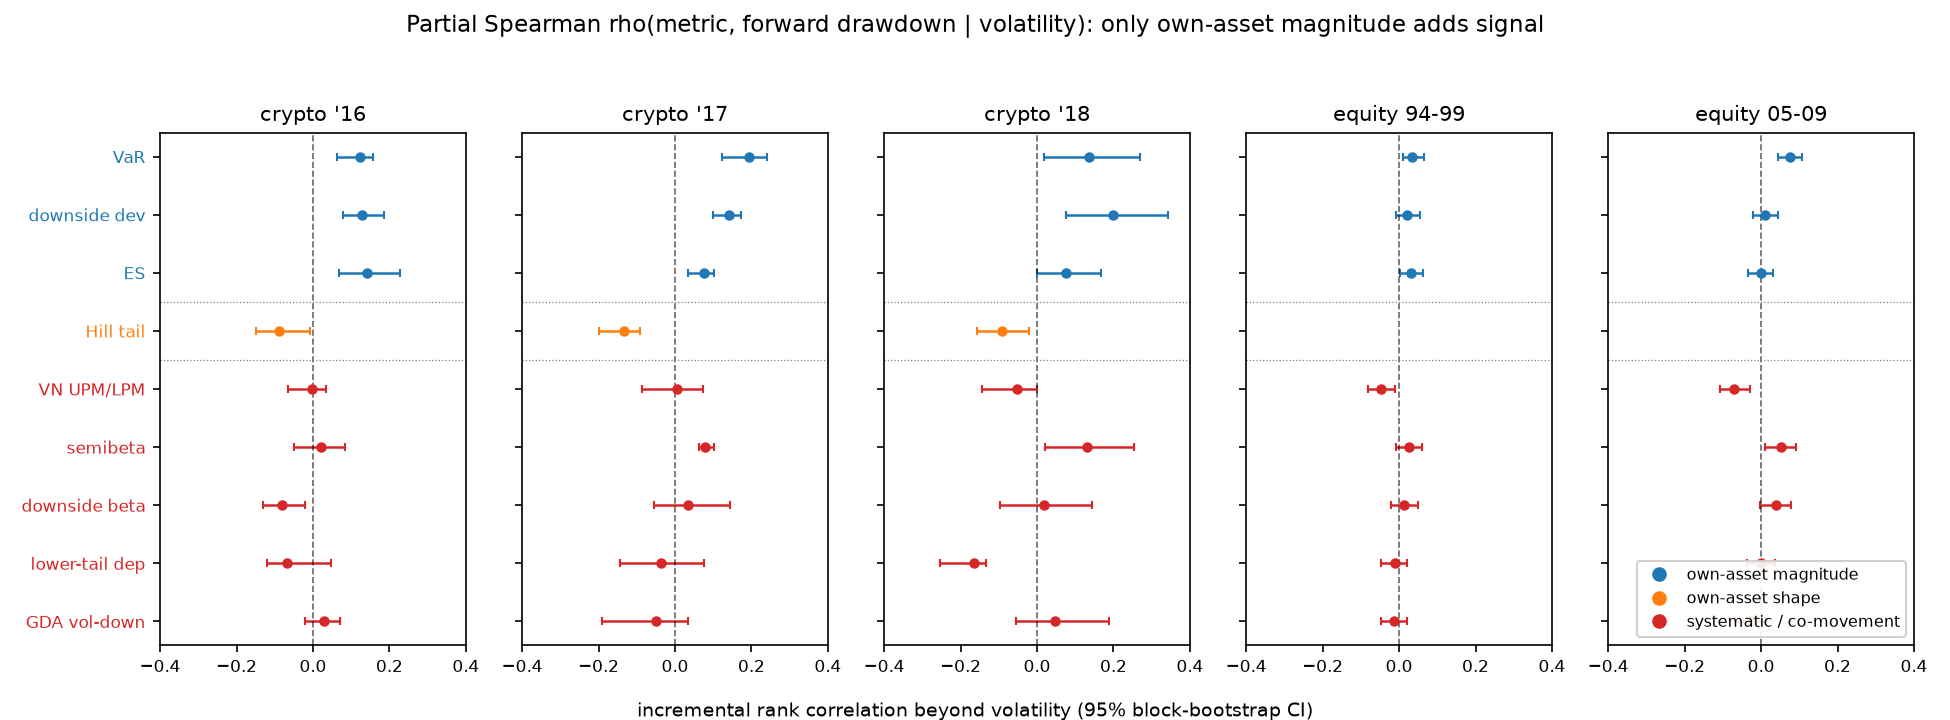
\includegraphics[width=\textwidth]{figures/fig1_partial_forest.png}
\caption{Incremental signal beyond volatility, by bed: partial Spearman
$\rho(\text{metric},\text{drawdown}\mid\text{volatility})$, grouped on both axes a
skeptic cares about, namely what the metric measures (magnitude vs shape) \emph{and}
whose distribution it uses (own-asset vs systematic co-movement with the market).
Only own-asset magnitude (blue) sits reliably right of zero. The lone own-asset
\emph{shape} metric, the Hill tail exponent (orange), is $\approx 0$ or negative,
so ``magnitude beats shape'' holds \emph{within} the own-asset family, and no
systematic co-movement metric (red) adds signal. Whiskers are $95\%$ block-bootstrap
CIs; dotted lines separate the three families.}
\label{fig:forest}
\end{figure*}

VaR is \emph{worse} than volatility
standalone on equity (Table~\ref{tab:h2h}) yet has a positive \emph{increment} there.
As a standalone ranker it is a noisier proxy for volatility, but the partial
correlation isolates its small orthogonal component. The increment is also larger where
markets are fat-tailed and blow-up-prone (crypto increments $0.12$--$0.19$, excess
kurtosis $8$--$21$, vs equity $0.03$--$0.08$; App.~\ref{app:hetero}).
Tail magnitude carries incremental information precisely when the tail is active.

One might object that drawdown is a magnitude-dominated statistic, so a magnitude
metric is bound to win. Expected maximum drawdown scales with $\sigma\sqrt{T}$~\cite{magdonismail2004},
so the objection is correct, and it is the point. Drawdown is the loss that ruins
investors, and the literature proposes shape metrics to forecast it. When we forecast
genuinely shape-sensitive targets instead, forward skew, downside fraction, and
tail-exceedance frequency, the shape metrics \emph{do} beat volatility on nearly every
bed, while volatility predicts them poorly (App.~\ref{app:target}). Shape metrics
forecast shape. Shape is simply not what drives drawdown.

\begin{table}[t]
\centering
\caption{Partial Spearman $\rho(\text{metric},\text{drawdown}\mid\text{volatility})$.
Rows 1--3 tail magnitude, rows 4--9 tail shape. $\ast$ survives BH ($q=0.05$,
positive); $\dagger$ survives BH negative; n/e = not estimable per date. Bold marks the highest value in each column.}
\label{tab:partials}
\small
\begin{tabular}{lccccc}
\toprule
Metric & cr-16 & cr-17 & cr-18 & eq 94 & eq 05 \\
\midrule
VaR & $+0.12\ast$ & $\mathbf{+0.19}\ast$ & $+0.13\ast$ & $\mathbf{+0.03}\ast$ & $\mathbf{+0.08}\ast$ \\
downside dev. & $+0.13\ast$ & $+0.14\ast$ & $\mathbf{+0.20}\ast$ & $+0.02$ & $+0.01$ \\
ES~\cite{rockafellar2000} & $\mathbf{+0.14}\ast$ & $+0.08\ast$ & $+0.08$ & $\mathbf{+0.03}$ & $+0.00$ \\
neg.\ semibeta~\cite{bpq2022} & $+0.02$ & $+0.08\ast$ & $+0.13\ast$ & $\mathbf{+0.03}$ & $+0.05\ast$ \\
UPM/LPM~\cite{violenawrocki2016} & $-0.00$ & $+0.01$ & $-0.05$ & $-0.05\dagger$ & $-0.07\dagger$ \\
downside beta~\cite{ang2006} & $-0.08\dagger$ & $+0.03$ & $+0.02$ & $+0.01$ & $+0.04$ \\
Hill tail~\cite{kellyjiang2014} & $-0.09\dagger$ & $-0.13\dagger$ & $-0.09\dagger$ & n/e & n/e \\
lower-tail dep.~\cite{chabiyo2018} & $-0.07$ & $-0.04$ & $-0.17\dagger$ & $-0.01$ & $+0.00$ \\
GDA~\cite{faragotedongap2018} & $+0.03$ & $-0.05$ & $+0.05$ & $-0.01$ & $-0.03$ \\
\bottomrule
\end{tabular}
\end{table}

%% =========================================================================
\section{Why volatility wins, and can anything beat it?}\label{sec:why}
\subsection{Persistence}
Volatility wins because it is \emph{persistent}, the founding
fact of ARCH/GARCH~\cite{engle1982,bollerslev1986}. Trailing volatility forecasts
forward volatility (rank correlation $0.42$--$0.84$), which in turn drives forward
drawdown. Table~\ref{tab:chain} decomposes this chain by bed. Both links exceed the
direct trailing-vol$\rightarrow$drawdown rank correlation they compose. We resist
calling forward volatility a
\emph{sufficient statistic}. A naive same-window mediation suggests it, but that test
is contaminated (forward volatility and drawdown share a window). Measured on a
disjoint, predictive window, trailing volatility retains a partial correlation of
$0.32$--$0.34$ on equity (Figure~\ref{fig:mediation}), so persistence is a
\emph{leading but incomplete} explanation, not a mechanism that reduces drawdown to
one number.

\begin{table}[t]
\centering
\caption{Persistence chain (mean per-date Spearman; all CIs exclude 0).}
\label{tab:chain}
\small
\begin{tabular}{lccc}
\toprule
Bed & trail$\rightarrow$fwd vol & fwd vol$\rightarrow$dd & (trail$\rightarrow$dd) \\
\midrule
crypto-16 & 0.68 & 0.77 & 0.62 \\
crypto-17 & 0.42 & 0.62 & 0.36 \\
crypto-18 & 0.42 & 0.53 & 0.38 \\
equity 94 & 0.84 & 0.71 & 0.61 \\
equity 05 & 0.80 & 0.70 & 0.56 \\
\bottomrule
\end{tabular}
\end{table}

\begin{figure}[t]
\centering
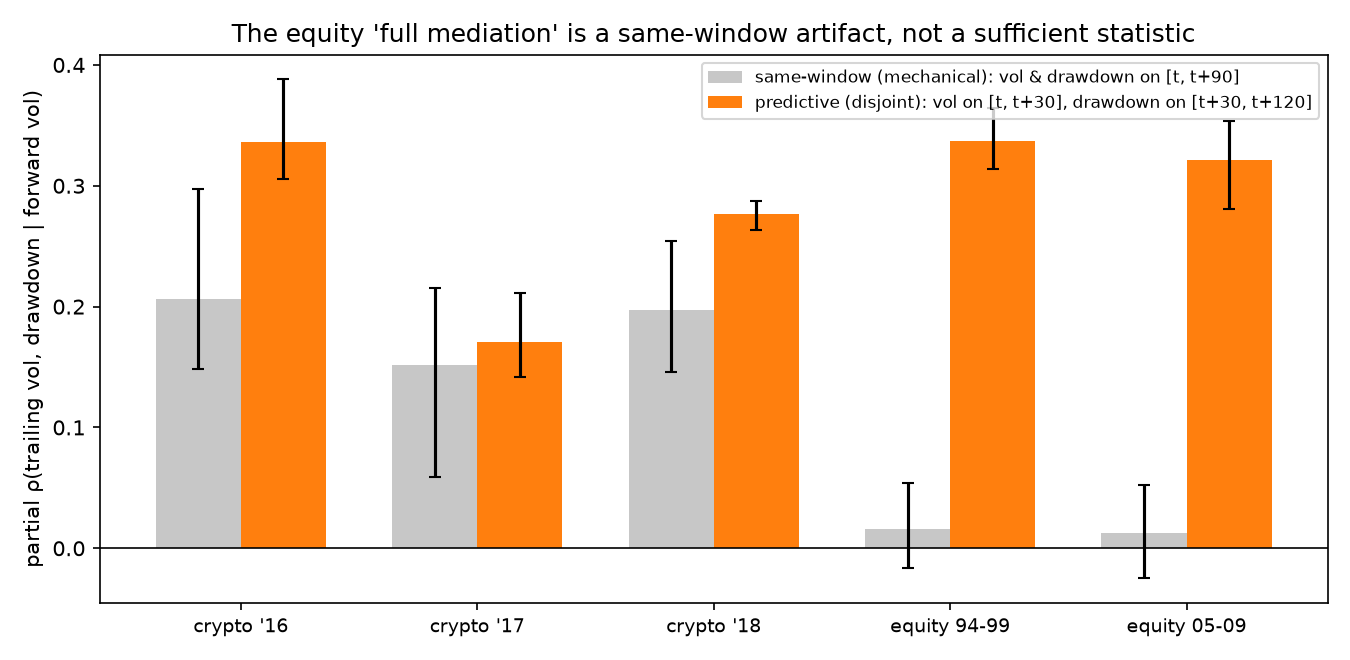
\includegraphics[width=\columnwidth]{figures/fig3_mediation.png}
\caption{Mediation: partial $\rho(\text{trailing vol},\text{drawdown}\mid
\text{forward vol})$. The same-window (mechanical) design gives $\approx 0$ on equity,
falsely suggesting full mediation. The predictive (disjoint-window) design gives
$0.32$--$0.34$, so forward volatility does not fully screen off trailing volatility.}
\label{fig:mediation}
\end{figure}

\subsection{Does the edge pay?}
A rank correlation is not a profit-and-loss statement.
The decomposition implies one natural composite, the equal-weight sum
$z(\text{vol})+z(\text{VaR})$ with no fitting, where $z(\cdot)$ is the cross-sectional
z-score (each metric standardized across the assets on a given date). We pre-registered
it. On a locked panel it shows \emph{no} significant out-of-sample gain over volatility
(Newey--West $t=0.67$, lag $3$), beating it only on fat-tailed crypto-bull
(Table~\ref{tab:econ}). A cost-aware tercile backtest agrees. The
high-risk tercile realizes $10$--$30$ percentage points more forward drawdown than the
low-risk tercile on every bed, net of a $20$~bps turnover cost, and the composite adds
nothing net of turnover except, again, on crypto-bull. Volatility is the workhorse.
Magnitude adds a little, and only where tails are fat.

\begin{table}[t]
\centering
\caption{Composite $z(\text{vol})+z(\text{VaR})$ vs.\ volatility: per-date Spearman
and difference (95\% CI); significant only on crypto-bull.}
\label{tab:econ}
\small
\begin{tabular}{lccc}
\toprule
Test bed & vol $\rho$ & comp $\rho$ & difference (95\% CI) \\
\midrule
crypto-16 & 0.62 & 0.62 & $-0.00$ (n.s.) \\
crypto-17 & 0.36 & 0.40 & $+0.05$ $[0.02,0.07]$ \\
crypto-18 & 0.38 & 0.39 & $+0.01$ (n.s.) \\
equity 94 & 0.61 & 0.60 & $-0.008$ $[-0.011,-0.004]$ \\
equity 05 & 0.56 & 0.56 & $-0.00$ (n.s.) \\
\midrule
\multicolumn{4}{l}{\emph{Locked panel:} $0.376 \rightarrow 0.388$, Newey--West $t=0.67$ (n.s.).}\\
\bottomrule
\end{tabular}
\end{table}

\subsection{Can a machine find more?}
If the residual is this small, a tireless automated
search should fail out-of-sample and merely overfit validation. We test this on a strict
train/validation/\emph{locked-test} split, the locked test scored once after the metric
is frozen. An LLM agent rewriting a scoring function and a $20{,}000$-configuration sweep
both inflate the best \emph{validation} score with search intensity while the
\emph{locked-test} score plateaus at the volatility baseline (Figure~\ref{fig:bon}).
Across $12$ holdout
panels $\times$ $3$ search seeds (App.~\ref{app:snooping}, a non-LLM generator at scale,
with the LLM loop as the single original panel), the validation-selected
metric's out-of-sample edge over volatility is at most $+0.07$ and averages
$+0.02$--$0.03$, straddling zero. No search, LLM or brute-force, finds a genuine
improvement. A non-LLM random sweep reproduces the plateau, so the danger is the cheap
search, not the language model. The statistics are classical data
snooping~\cite{white2000,bailey2017}; what is new is that an autonomous agent removes
the last brake on trial count (analyst effort), so a locked, survivorship-free
holdout scored exactly once becomes mandatory, not merely advisable.

\subsection{What volatility is for?}
The clearest positive use is forecasting outright
blow-ups. On the locked crypto test, volatility predicts which assets crater (forward
return $\le -80\%$) with ROC-AUC $0.68$ ($0.95$
for the stricter $\le -90\%$ cutoff) and a $2.5\times$
top-decile lift, while a gradient-boosting model over all ten metrics, chosen on
validation (AUC $0.73$), overfits and loses on the locked test (AUC $0.59$). The
blow-up base rate is only ${\approx}1.2\%$, so these AUCs are noisy and we read them as
ordinal. Again the \emph{size}, not the shape, of recent moves carries the
signal. This is a ranking result, not a deployment recommendation (cost, liquidity, and
reflexivity frictions are unmodeled).

\begin{figure*}[t]
\centering
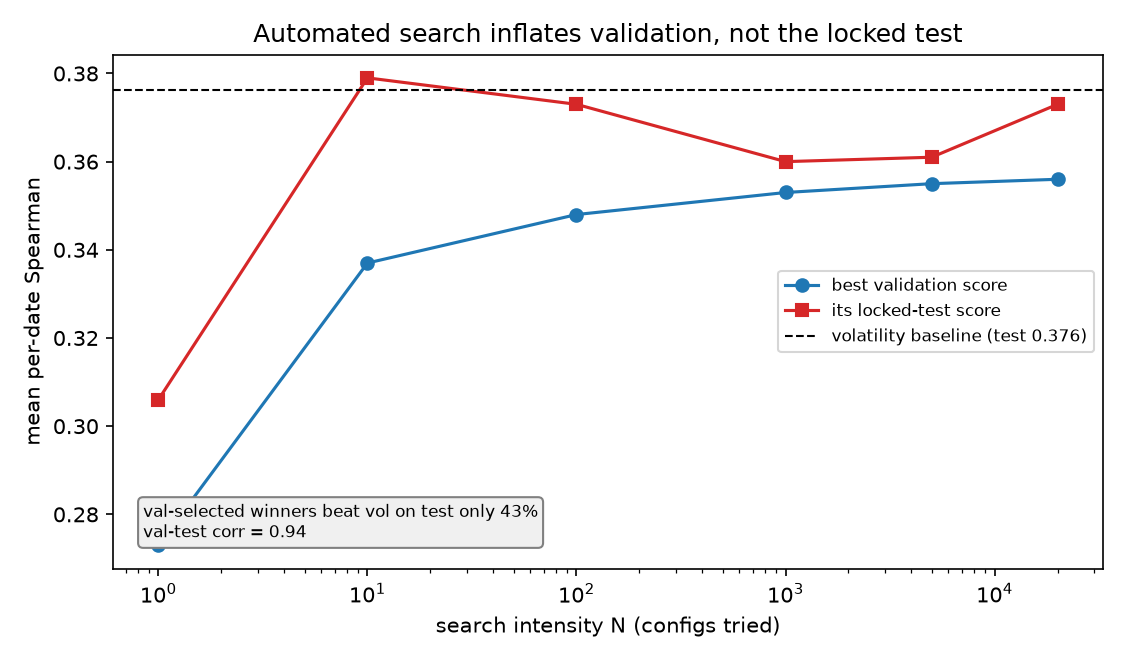
\includegraphics[width=0.7\textwidth]{figures/fig5_best_of_N.png}
\caption{Automated discovery cannot beat volatility out of sample. As search intensity
grows, the best \emph{validation} score climbs while its locked-\emph{test} score stays
flat at the volatility baseline. On this ($2017\!\to\!2018$-crash) holdout,
validation-selected winners beat volatility on the locked test only $43\%$ of the time;
across $12$ panels $\times$ $3$ seeds the win-rate is regime-dependent, but the
locked-test edge over volatility never exceeds noise (App.~\ref{app:snooping}).}
\label{fig:bon}
\end{figure*}

%% =========================================================================
\section{Discussion and conclusion}\label{sec:discussion}
The pieces form one coherent picture. Volatility sets a high bar because it is
persistent (\S\ref{sec:why}). The only thing left to add is the magnitude of tail
losses, and only a little, mostly in fat-tailed markets (\S\ref{sec:magnitude}). So no
standalone metric beats volatility (\S\ref{sec:verdict}), a pre-registered composite
yields no significant out-of-sample gain, automated search cannot find one, and the
economics track the statistics (\S\ref{sec:why}). The recurring
failure of \emph{asymmetry} and \emph{shape}
metrics (including the partial-moment ratio~\cite{violenawrocki2016}) is
not an implementation accident. Once symmetric volatility is accounted for, the
asymmetric structure adds no incremental cross-sectional information for
forecasting drawdown. The fair-field disciplines change what one would \emph{report}, not the verdict.
Survivorship bias alone flips a co-crash shape metric from significantly worse than
volatility to a tie and inflates the apparent magnitude edge (App.~\ref{app:ablation}),
yet the verdict that no shape metric beats volatility is robust to dropping any single
discipline. The disciplines guard the honesty of the numbers, not the direction of the
conclusion. We are deliberately careful about the \emph{strength} of the
persistence story. An earlier version of this project claimed forward volatility
was a sufficient statistic, found that claim was a same-window measurement
artifact, and retracted it here, just as an earlier ``survivorship masks
downside value'' thesis was retracted when a hardened test refuted it. The paper
reports only claims that survived stress-testing.

The practical takeaway is unglamorous but firm. For cross-sectional drawdown
forecasting, use volatility (optionally with a small tail-magnitude term in
fat-tailed markets) and treat any downside metric ``discovered'' to beat it,
by hand or by machine, as unproven until it clears a locked, survivorship-free
holdout. On a level field, volatility is not glamorous, but it is very hard to beat.

\textbf{Limitations.} The performance measure is rank correlation, not a full tradable P\&L
(\S\ref{sec:why} is a first economic check, not a portfolio study); the
crypto beds have few formation dates ($7$--$9$), so their significance is
suggestive and the null ``shape adds nothing'' leans on the well-powered equity
beds; and the repurposed pricing metrics are daily adaptations, so results speak to
drawdown forecasting, not the originals' pricing claims.

%% =========================================================================
\begin{thebibliography}{99}
\small
\bibitem{andersen2003} T.~Andersen, T.~Bollerslev, F.~Diebold, and P.~Labys.
Modeling and forecasting realized volatility. \emph{Econometrica}, 71(2):579--625, 2003.
\bibitem{ang2006} A.~Ang, J.~Chen, and Y.~Xing. Downside risk.
\emph{Review of Financial Studies}, 19(4):1191--1239, 2006.
\bibitem{atilgan2020} Y.~Atilgan, T.~Bali, K.~Demirtas, and A.~Gunaydin.
Left-tail momentum. \emph{Journal of Financial Economics}, 135(3):725--753, 2020.
\bibitem{bailey2014} D.~Bailey and M.~L\'opez de Prado. The deflated Sharpe ratio.
\emph{Journal of Portfolio Management}, 40(5):94--107, 2014.
\bibitem{bailey2017} D.~Bailey, J.~Borwein, M.~L\'opez de Prado, and Q.~Zhu.
The probability of backtest overfitting.
\emph{Journal of Computational Finance}, 20(4):39--70, 2017.
\bibitem{bawa1975} V.~Bawa. Optimal rules for ordering uncertain prospects.
\emph{Journal of Financial Economics}, 2(1):95--121, 1975.
\bibitem{bollerslev1986} T.~Bollerslev. Generalized autoregressive conditional
heteroskedasticity. \emph{Journal of Econometrics}, 31(3):307--327, 1986.
\bibitem{bpq2022} T.~Bollerslev, A.~Patton, and R.~Quaedvlieg. Realized semibetas.
\emph{Journal of Financial Economics}, 144(1):227--246, 2022.
\bibitem{chabiyo2018} F.~Chabi-Yo, S.~Ruenzi, and F.~Weigert. Crash sensitivity and
the cross-section of expected stock returns.
\emph{Journal of Financial and Quantitative Analysis}, 53(3):1059--1100, 2018.
\bibitem{chekhlov2005} A.~Chekhlov, S.~Uryasev, and M.~Zabarankin. Drawdown measure
in portfolio optimization. \emph{International Journal of Theoretical and Applied
Finance}, 8(1):13--58, 2005.
\bibitem{corsi2009} F.~Corsi. A simple approximate long-memory model of realized
volatility. \emph{Journal of Financial Econometrics}, 7(2):174--196, 2009.
\bibitem{engle1982} R.~Engle. Autoregressive conditional heteroscedasticity with
estimates of the variance of U.K.\ inflation. \emph{Econometrica}, 50(4):987--1007, 1982.
\bibitem{faragotedongap2018} A.~Farago and R.~T\'edongap. Downside risks and the
cross-section of asset returns.
\emph{Journal of Financial Economics}, 129(1):69--86, 2018.
\bibitem{frazzinipedersen2014} A.~Frazzini and L.~Pedersen. Betting against beta.
\emph{Journal of Financial Economics}, 111(1):1--25, 2014.
\bibitem{fishburn1977} P.~Fishburn. Mean-risk analysis with risk associated with
below-target returns. \emph{American Economic Review}, 67(2):116--126, 1977.
\bibitem{harvey2016} C.~Harvey, Y.~Liu, and H.~Zhu. $\ldots$ and the cross-section
of expected returns. \emph{Review of Financial Studies}, 29(1):5--68, 2016.
\bibitem{kellyjiang2014} B.~Kelly and H.~Jiang. Tail risk and asset prices.
\emph{Review of Financial Studies}, 27(10):2841--2871, 2014.
\bibitem{leviwelch2020} Y.~Levi and I.~Welch. Symmetric and asymmetric market betas
and downside risk. \emph{Review of Financial Studies}, 33(6):2772--2795, 2020.
\bibitem{magdonismail2004} M.~Magdon-Ismail, A.~Atiya, A.~Pratap, and
Y.~Abu-Mostafa. On the maximum drawdown of a Brownian motion.
\emph{Journal of Applied Probability}, 41(1):147--161, 2004.
\bibitem{moreiramuir2017} A.~Moreira and T.~Muir. Volatility-managed portfolios.
\emph{Journal of Finance}, 72(4):1611--1644, 2017.
\bibitem{rockafellar2000} R.~T.~Rockafellar and S.~Uryasev. Optimization of
conditional value-at-risk. \emph{Journal of Risk}, 2(3):21--41, 2000.
\bibitem{sortino1991} F.~Sortino and R.~van der Meer. Downside risk.
\emph{Journal of Portfolio Management}, 17(4):27--31, 1991.
\bibitem{violenawrocki2016} F.~Viole and D.~Nawrocki. Predicting risk/return
performance using upper partial moment/lower partial moment metrics.
\emph{Journal of Mathematical Finance}, 6(5):900--920, 2016.
\bibitem{white2000} H.~White. A reality check for data snooping.
\emph{Econometrica}, 68(5):1097--1126, 2000.
\end{thebibliography}

%% =========================================================================
\appendix
\section{Reproducibility}\label{app:repro}
Code, data pointers, and result logs to reproduce every table and figure are
available at \url{https://github.com/meghanadhpulivarthi/downside-risk-metrics-study}.
The data sources are a CoinMarketCap daily
crypto dump (retaining delisted coins), yfinance S\&P~500 constituents and the
market index, and point-in-time index membership.

\section{Power and placebo}\label{app:partials}
The partial correlations of Table~\ref{tab:partials} (\S\ref{sec:magnitude}) survive BH
on the beds marked; the one equity ES cell that is nominally significant does not survive
correction. We also report power on the thin crypto beds. For VaR, on crypto-16 ($n=8$) and crypto-17 ($n=9$)
the effect ($0.12$, $0.19$) exceeds the $80\%$-power minimum detectable effect
($0.09$, $0.09$) and is stable under leave-one-date-out; on crypto-18 ($n=7$) the
effect ($0.13$) is below its MDE ($0.18$) and is reported as suggestive. A placebo
(permuting forward drawdown within each date) drives the trailing-volatility
correlation to $\approx 0$ on four of five beds; the exception, crypto-18
($+0.028$, CI $[0.003,0.059]$), is negligible against a real rank correlation of $\approx
0.38$ and reflects the coarse block bootstrap at $n=7$. On the well-powered equity beds
the $80\%$-power minimum detectable increment for the shape metrics is $0.034$--$0.042$,
and the observed shape increments sit at or below it (Table~\ref{tab:partials}), so on
equity ``shape adds nothing'' is a powered null rather than a failure to detect.

\section{The persistence chain}\label{app:chain}
Table~\ref{tab:chain} (\S\ref{sec:why}) decomposes why trailing volatility forecasts
drawdown. The forward-vol$\rightarrow$drawdown column is contemporaneous (both over the
same forward window) and hence partly mechanical~\cite{andersen2003}; the genuinely
predictive link is trailing$\rightarrow$forward volatility. Figure~\ref{fig:chain} shows
the two links relative to the direct trailing-volatility$\rightarrow$drawdown rank
correlation, by bed.

\begin{figure}[t]
\centering
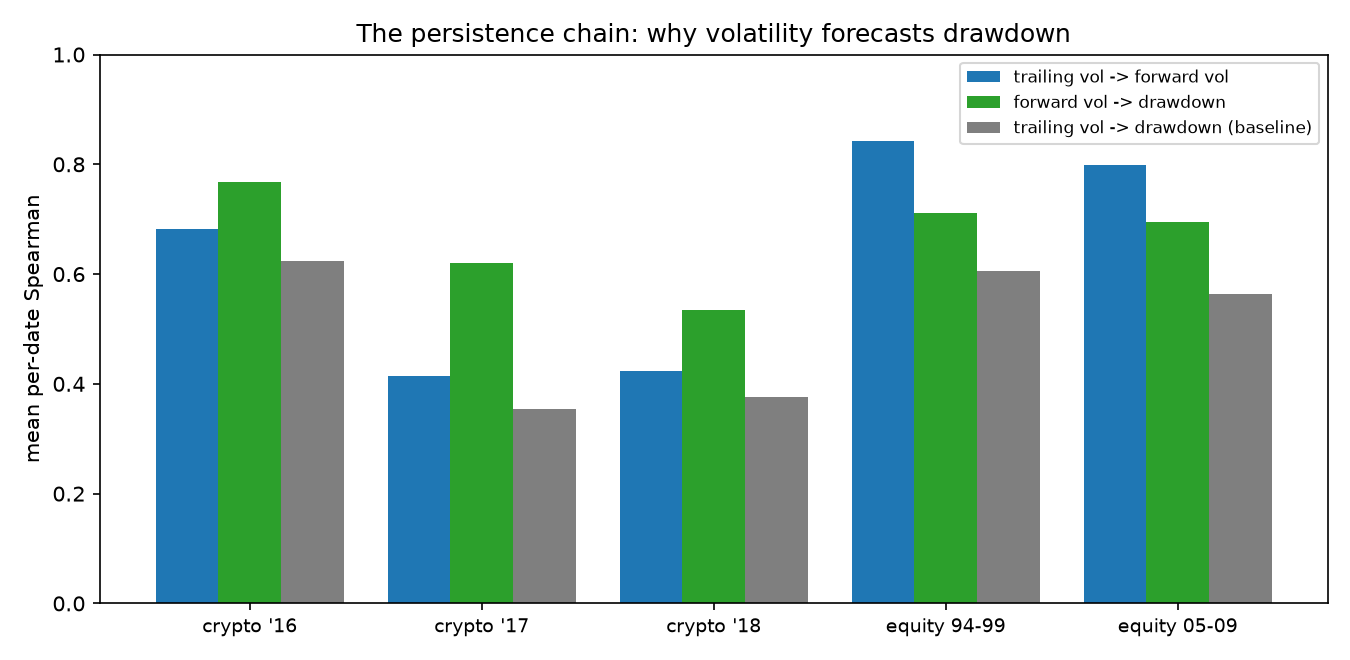
\includegraphics[width=\columnwidth]{figures/fig2_persistence_chain.png}
\caption{The two links of the persistence chain relative to the direct
trailing-volatility$\rightarrow$drawdown rank correlation, by bed.}
\label{fig:chain}
\end{figure}

\section{Mediation: forward volatility is not a sufficient statistic}\label{app:mediation}
It is tempting to claim drawdown predictability simply \emph{is} volatility
persistence, meaning that forward volatility is a sufficient statistic. A naive mediation
test seems to confirm it. Controlling for forward volatility, trailing volatility's
partial correlation with drawdown collapses to $\approx0$ on equity. But that test is
contaminated. Forward volatility and forward drawdown are measured over the \emph{same}
window, so conditioning on one mechanically absorbs the other. Measuring the mediator on
a \emph{disjoint, earlier} window (volatility over days $1$--$30$, drawdown over days
$31$--$120$, so it is genuinely predictive), the mediation vanishes. Trailing
volatility retains a partial correlation of $0.32$--$0.34$ on equity
(Figure~\ref{fig:mediation}). Trailing volatility carries forecasting content a
short-horizon volatility forecast does not, so persistence is a leading but incomplete
explanation. Because the disjoint mediator is a noisy $30$-day volatility proxy,
measurement error could inflate this residual, so we read it as consistent with
incomplete mediation rather than proof that forward volatility is insufficient.
Consistently, drawdown rank correlation and volatility persistence rise and fall
together as the horizon varies (App.~\ref{app:horizon}). The mediation figure is
Figure~\ref{fig:mediation} in \S\ref{sec:why}.

\section{Horizon dynamics}\label{app:horizon}
Sweeping the forecast horizon from $14$ to $90$ days, volatility persistence and
drawdown rank correlation move together (Figure~\ref{fig:horizon}). On equity both rise
(persistence $0.66\rightarrow0.84$, rank correlation $0.47\rightarrow0.61$, at a roughly
constant gap), while on crypto both are flat. Wherever persistence is higher, so is the
rank correlation, consistent with persistence driving most of the forecastable variation,
with the constant gap the part it does not explain.

\begin{figure*}[t]
\centering
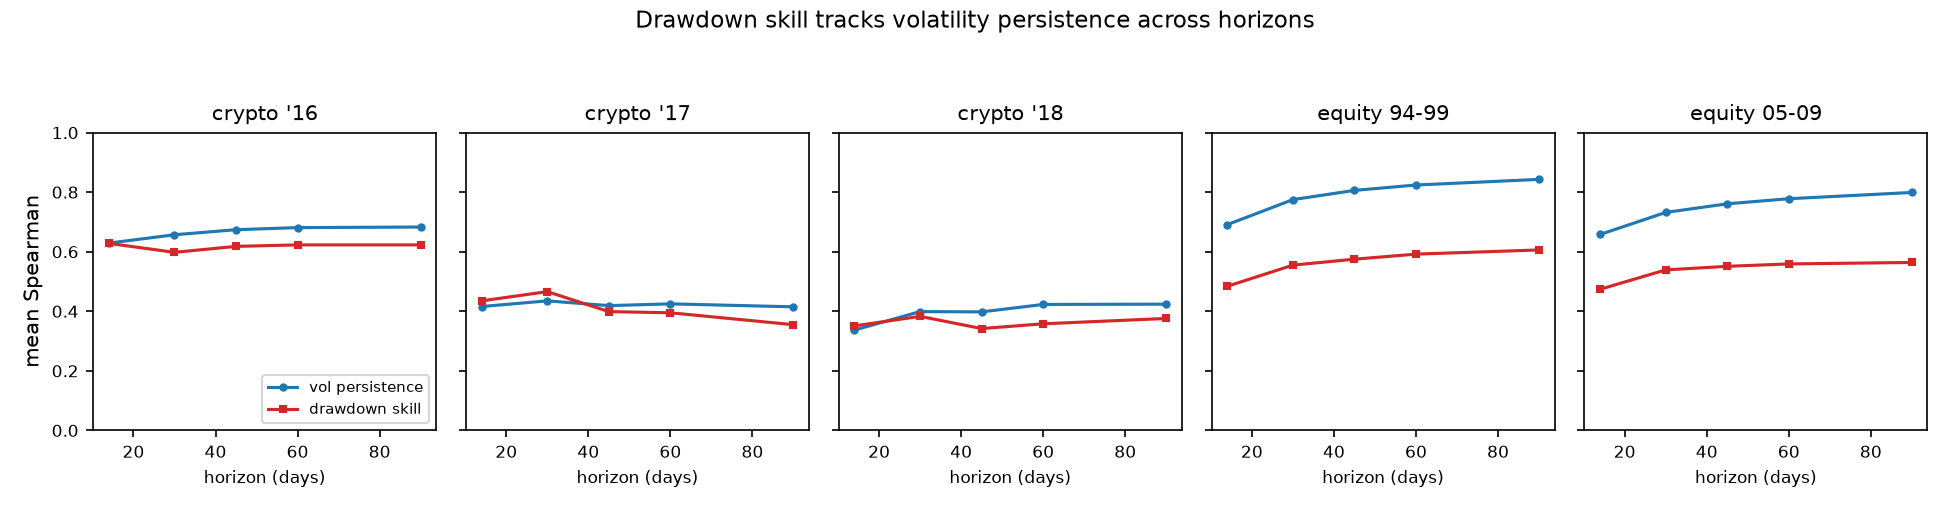
\includegraphics[width=\textwidth]{figures/fig4_horizon_decay.png}
\caption{Volatility persistence (blue) and drawdown-forecast rank correlation (red) versus
forecast horizon, by bed. The curves track.}
\label{fig:horizon}
\end{figure*}

\section{When the magnitude increment is largest}\label{app:hetero}
Is the VaR increment genuinely larger where tails are fatter, or does it only look
that way across five points? We regress each formation date's VaR increment, the partial
$\rho(\text{VaR},\text{drawdown}\mid\text{volatility})$, on that date's cross-sectional
tail-fatness, pooling all $144$ dates across the five beds. Because the relationship is
fundamentally between beds, the honest test clusters by bed, where the slope is positive
but only suggestive at five clusters (median excess kurtosis $p\approx0.10$, blow-up rate
$p\approx0.15$). Treating the $144$ dates as independent, which they are not, the same
slopes ($+0.013$ for kurtosis, $+0.76$ for blow-up rate) exclude zero, so the
within-regime relationship is consistent even where the between-bed test is underpowered.
Figure~\ref{fig:hetero} shows the per-bed picture, with the increment concentrated in the
fat-tailed crypto beds.

The same pattern holds \emph{within} crypto. Splitting the crypto dates at their median
aggregate (cross-sectional-median) volatility, the VaR increment rises from $+0.13$
(CI $[0.06,0.18]$) on low-stress dates to $+0.18$ ($[0.09,0.24]$) on high-stress dates
($24$ dates, $12$ per regime; suggestive given the overlap), while on equity it is flat
and small ($+0.056$ vs.\ $+0.050$; $120$ dates). Tail magnitude carries incremental
information precisely when the tail is active.

\begin{figure}[t]
\centering
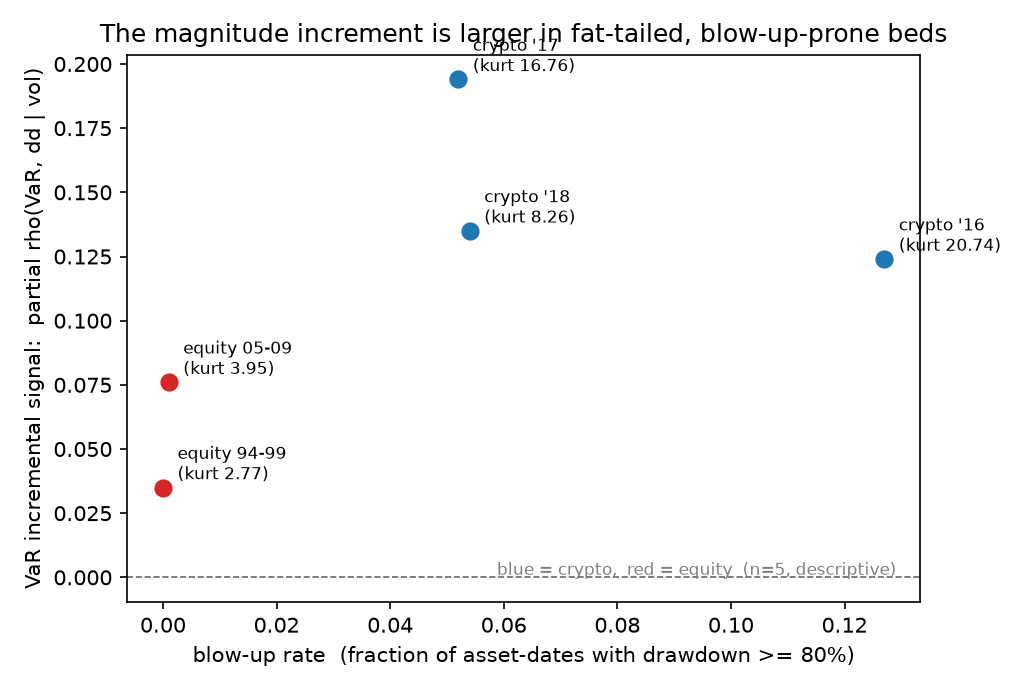
\includegraphics[width=\columnwidth]{figures/fig6_increment_vs_tailfat.png}
\caption{VaR incremental signal (partial $\rho\mid$ volatility) versus blow-up
rate, by bed. Behind it, a pooled per-date regression across all $144$ dates gives a
positive slope whose date-level CI excludes zero, suggestive when clustered by bed.}
\label{fig:hetero}
\end{figure}

\section{Delisting-coding robustness}\label{app:delisting}
The crypto forward-drawdown codes a mid-window delisting as a terminal $-100\%$ loss.
To confirm the magnitude increment is a genuine crash-severity signal, not an artifact
of that code, nor a restatement of the blow-up result (\S\ref{sec:why}), we
recompute $\rho(\text{metric},\text{drawdown}\mid\text{vol})$ under two alternative
codings. The first values a delisted asset at its \emph{last traded price} (ordinary
peak-to-trough, no $-100\%$ override). The second \emph{excludes} delisted assets (rank
correlation among survivors only). Within the point-in-time top-$100$ universe, mid-window
delistings are rare ($0.9\%$ of asset-dates on crypto-2016 and none on the other
four beds), so the three codings barely differ. VaR's increment is unchanged to
within $\pm0.02$ across all three (Table~\ref{tab:delisting}); downside deviation and
ES behave identically. The magnitude edge is drawdown-\emph{severity} forecasting,
distinct from the terminal-death signal.

\begin{table}[h]
\centering
\small
\caption{VaR partial $\rho(\text{VaR},\text{drawdown}\mid\text{vol})$ under three
delisting codings. Baseline and last-price coincide (mid-window delistings are rare);
the increment is unchanged to within $\pm0.02$.}
\label{tab:delisting}
\begin{tabular}{lccc}
\toprule
Bed & baseline ($-100\%$) & last-price & exclude \\
\midrule
crypto-16 & $+0.12$  & $+0.12$  & $+0.14$  \\
crypto-17 & $+0.19$  & $+0.19$  & $+0.19$  \\
crypto-18 & $+0.14$  & $+0.14$  & $+0.14$  \\
equity-94 & $+0.035$ & $+0.035$ & $+0.035$ \\
equity-05 & $+0.076$ & $+0.076$ & $+0.076$ \\
\bottomrule
\end{tabular}
\end{table}

\section{Pre-registered composite and economic backtest}\label{app:composite}
The composite is $z(\text{vol})+z(\text{VaR})$, equal weight, computed
cross-sectionally per date, with no fitting. VaR was chosen a priori as the
magnitude metric surviving correction on all five beds (\S\ref{sec:magnitude}); the
weights are untuned, so the fully out-of-sample evidence is the locked-panel test
(Table~\ref{tab:econ}, \S\ref{sec:why}), which is not significant. The economic backtest
(Figure~\ref{fig:economic}) sorts the universe into risk
terciles and measures realized-drawdown discrimination (forward DD of the high-
minus low-risk tercile) and the forward-return spread, net of a $20$~bps turnover
cost.

\begin{figure}[t]
\centering
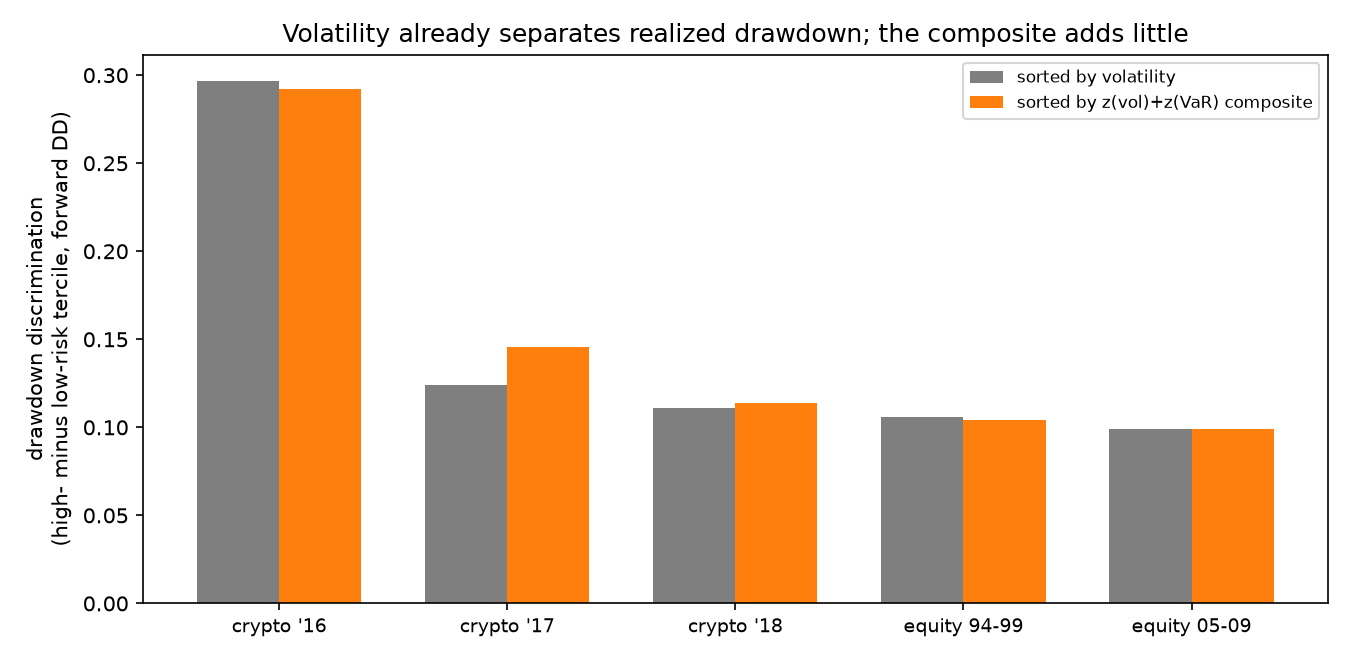
\includegraphics[width=\columnwidth]{figures/fig7_economic.png}
\caption{Realized drawdown discrimination (high- minus low-risk tercile) by bed,
sorting on volatility vs.\ the composite. Volatility already separates drawdown
strongly; the composite is indistinguishable except marginally on crypto-bull.}
\label{fig:economic}
\end{figure}

\section{Disciplines ablation}\label{app:ablation}
Each of the three fair-field disciplines materially affects the reported results. We
ask which shape metric one would have credited without each.

\emph{Without survivorship-free data.} We rebuild the crypto universe survivors-only,
keeping at each formation date only coins that neither delisted nor crashed to dust
(ended below $5\%$ of their all-time peak) by
the panel end. About a third of the point-in-time top $100$ survive. On the $2018$
crash bed this flips negative semibeta, a co-crash shape metric, from a head-to-head
$-0.067$ against volatility (CI $[-0.131,-0.003]$, significantly worse) to $+0.055$
(CI $[-0.082,0.178]$, a statistical tie); downside beta closes from $-0.23$ to $-0.01$
over the same change, and VaR's partial rises from $+0.135$ to $+0.205$. Survivorship
bias erases shape's penalty and inflates the magnitude edge, and it does so precisely in
the crash regime, where hiding the coins that died most reshapes the cross-section. On
the calm and bull crypto beds the shift is small and mixed. It does not manufacture a
winner. No shape metric significantly beats volatility even survivors-only, and the rest
stay far below it, the Viole--Nawrocki ratio near $-1.2$ and lower-tail dependence near
$-1.1$.

\emph{Without multiple-testing correction.} Across the ${\sim}45$ head-to-head cells the
only metrics nominally beating volatility at $p<0.05$ are downside deviation and VaR,
both tail-magnitude measures, and only on the crypto-bull bed. No shape metric is even
nominally positive, so Benjamini--Hochberg is not what holds shape back.

\emph{Without a locked holdout.} The discovery experiment (App.~\ref{app:snooping})
makes this concrete. A validation-selected metric's inflated validation score reads as
a win, while its once-scored locked-test score sits at the volatility baseline.

The disciplines change what one would \emph{report}, not the verdict. Even stripped of
every guardrail, no shape metric beats volatility.

%% =========================================================================
\section{Target sensitivity}\label{app:target}
Drawdown is a magnitude-dominated statistic, so one might ask whether
``magnitude beats shape'' is forced by the target. We re-score every metric against
shape-sensitive forward targets, namely forward return skew (sign-flipped so higher is more
left-asymmetric), the forward downside fraction (forward downside deviation over
forward volatility, which is scale-free), and the forward tail-exceedance frequency
(share of forward days below the trailing fifth percentile).

The picture inverts by target (Table~\ref{tab:target}). On the magnitude target,
volatility wins on all five beds and no shape metric beats it. On every shape-sensitive
target, volatility's rank correlation is near zero or negative, and the shape metrics
beat it on nearly every bed. The Viole--Nawrocki ratio, the Hill exponent, both
semibetas, downside beta, lower-tail dependence, and the disappointment-aversion proxy
all forecast forward shape better than volatility does. The shape metrics are therefore
not mis-implemented or strawmanned; they carry genuine shape information. They add
nothing to drawdown forecasting because drawdown is a magnitude phenomenon and shape
is not what drives it.

These are daily adaptations of metrics built at other horizons, and two deserve a note.
Our per-asset Hill loss-tail exponent is a simplification of the Kelly--Jiang common tail
factor, which is estimated from the pooled cross-section. We compute it per asset for a
like-for-like per-date comparison. The Viole--Nawrocki upper-to-lower partial-moment ratio
is high when upside dominates downside, so its negative correlation with drawdown is
expected by construction, and the finding is that its \emph{increment} beyond volatility
is zero, not that its sign is wrong. That every shape metric forecasts forward shape
(above) is direct evidence the adaptations are faithful rather than strawmen. Downside
deviation, our operationalization of the Sortino and Bawa--Fishburn semi-deviation, is
the lower partial moment of order two about a zero target.

\begin{table}[h]
\centering
\small
\caption{Winner by forward target. Volatility wins the magnitude target; shape metrics
win every shape-sensitive target.}
\label{tab:target}
\begin{tabular}{lcc}
\toprule
Forward target & vol rank corr (range) & shape beats vol \\
\midrule
max drawdown (magnitude) & $+0.36$ to $+0.62$ & none, any bed \\
$-$skew (shape) & $-0.21$ to $-0.07$ & most, every bed \\
downside fraction (shape) & $-0.25$ to $-0.05$ & most, every bed \\
tail-exceedance freq (shape) & $-0.52$ to $-0.10$ & most, every bed \\
\bottomrule
\end{tabular}
\end{table}

%% =========================================================================
\section{Automated discovery: best-of-$N$ and robustness}\label{app:snooping}
On the original locked panel, both the LLM loop and the $20{,}000$-config sweep inflate
the best \emph{validation} score with search intensity while the locked \emph{test}
score stays flat at the volatility baseline (Table~\ref{tab:bon}, Figure~\ref{fig:bon}).
Validation-selected winners beat volatility on the locked test only $43\%$ of the time
(directed search) despite a $0.94$ validation--test rank correlation.

\begin{table}[h]
\centering
\caption{Best-of-$N$ discovery. Validation inflates with search intensity; the
locked test does not (volatility baseline $0.376$). Validation and test are
different splits, so compare trends, not levels.}
\label{tab:bon}
\small
\begin{tabular}{rcc}
\toprule
Search intensity $N$ & Best validation & Its locked test \\
\midrule
1 & 0.27 & 0.31 \\
100 & 0.35 & 0.37 \\
20{,}000 & 0.356 & 0.373 \\
\bottomrule
\end{tabular}
\end{table}

To check that this is not a single-panel artifact, we re-ran the
candidate search (a general nonlinear generator over per-date feature ranks, $1{,}500$
candidates per run) over a grid of holdout panels $\times$ $3$ search seeds, in two
families: \emph{out-of-time}, a fixed-length test window slid through the timeline
with validation always chronologically earlier (six windows, including the original
$2017\!\to\!2018$ split); and \emph{random}, order-ignoring $10$-val/$7$-test
repartitions of the non-train dates (six draws). Per run we record the
validation-selected metric's locked-test edge over volatility (\emph{test gap}) and the
fraction of validation-winners that also beat volatility on test (\emph{win-rate}).

\emph{The plateau is stable.} The test gap averages $+0.020$ (out-of-time; range
$-0.028$ to $+0.046$) and $+0.035$ (random; $+0.014$ to $+0.072$), always small and
often straddling zero, so no search beats volatility out-of-sample by more than noise on
any panel or seed. Validation--test rank correlation is $0.94$--$0.99$ throughout.
\emph{The win-rate is not.} It averages $0.79$ (out-of-time, range $0.55$--$1.00$) and
$0.82$ (random, $0.62$--$0.97$), lowest on holdouts where volatility's own rank correlation is high
on the test (the $2018$ crash, $0.43$ directed / $0.57$ milder generator) and near $1.0$
on calm windows. Because these nominal ``wins'' come with a test gap of essentially
zero, the \emph{sign} of the win-rate is far less informative than its \emph{magnitude}.
The validation-selected metric matches, but does not beat, volatility.

\end{document}
